% Evaluation assembled from completed evidence only, 2026-11-03.
% No new Callisto runs, tuning/selection or PDF compilation is required.
\section{Evaluation}
\label{sec:evaluation}

The evaluation addresses three questions. First, does the implementation
respect the PI calibration and initialization derived in
Section~\ref{sec:fpi_controller}? Second, are the reference-model
calculations consistent with the implemented nonlinear rule law? Third,
how does the full Fuzzy controller compare with fixed PI baselines under
post-centering delivery disturbances in continuous-phase Callisto?
These questions require separate evidence: implementation equivalence,
reference-model consistency, and finite-horizon performance do not
establish the same claim.

\subsection{Evidence groups and comparison design}
\label{subsec:eval_design}

We use three completed actual-Callisto campaigns, denoted M0, M2 and M3,
and separate fluid-reference calculations. M0 comprises six PI/linear-
counterpart pairs, or 12 actual runs. M2 comprises four actual runs:
PI and full Fuzzy, each with a clean trace and a single-edge latency
burst. M3 comprises 180 actual validation runs: 30 independent paired
seeds, two random-latency regimes and three fixed controllers. Six M3
pilot runs are separate from the 180-run validation and are not treated
as independent test replications. Reference calculations are not added
to the actual-Callisto run count.

The primary performance comparison is moderate PI against the full
Fuzzy law calibrated to its PI gain coordinates. M3 additionally includes
a prespecified stronger PI candidate. All candidates are frozen within
these campaigns. The linear surface $F_0$ is used only for the M0
implementation check and explicitly labeled same-input diagnostics;
M2 and M3 execute the full 25-rule nonlinear law. Axis matching controls
scales and update conventions, but is not an assertion that either
candidate is the best independently tuned controller.

\subsection{Continuous Callisto setup and delivery disturbances}

M2 and M3 use the continuous oscillator phases, local-clock scheduling
and integer receiving-buffer counts described in
Section~\ref{sec:fpi_controller}. Table~\ref{tab:eval_setup} gives their
common configuration. Reported token counts represent counted frames
in this model. There is no shared physical controller grid in
these actual runs. The fixed native integration scale is
$h=p/\omega_{\rm base}$, with the same convention in the calibrated
Fuzzy controller. The initial intrinsic-frequency spread is 400 ppm of
the normalized frequency unit.

\begin{table*}[t]
\caption{Common configuration of the aligned burst and random-latency experiments.
Time is measured in physical reference ticks unless specified as local ticks.}
\label{tab:eval_setup}
\centering
\begin{tabular}{@{}ll@{}}\toprule
Parameter & Value\\\midrule
Network & Three-node bidirectional triangle; six receiving buffers\\
Intrinsic frequencies $\omega^u$ & $(1.0002,0.9998,0.9999)^\top$\\
Initial phases; implementation base frequency & $0.1$ at every node; $\omega_{\rm base}=29999/30000$\\
Capacity; initial occupancy; target & $C=2048$; $\beta_e(0)=\beta_e^*=1024$ frames\\
Initial in-flight frames; delayed-run marking & 20 per channel; 1044 in the recorded convention\\
Nominal physical path delay & 20\\
Polling; control-execution delay & $p=1000$; $d_{\rm ctrl}=10$ local ticks\\
Moderate PI $(k_p,k_i)$ & $(2\times10^{-6},5\times10^{-11})$\\
Stronger fixed PI, M3 only & $(4\times10^{-6},5\times10^{-11})$\\
Full Fuzzy $(K_e,K_{\Delta e},K_u)$ & $(0.1,3.9998666667,-4.0961365379\times10^{-5})$\\
Execution policy & $u_{\max}=0.01$; shared guards enabled; reserve zero; no anti-windup\\
Optional mechanisms & Observer and supervisory mode switching disabled\\
Horizon; disturbance onset & $4\times10^6$; $t_{\rm on}=2\times10^6$\\\bottomrule
\end{tabular}
\end{table*}

\paragraph{Burst after nominal centering.}
In M2, desired send-time latency on one directed channel, identified as
$1\to2$ in the runtime configuration, changes from 20 to 40 during
$[2\times10^6,2.1\times10^6)$ and returns to 20 afterwards. All other
channels remain at 20. Each controller has its own clean counterfactual
with latency 20 throughout. A controller's burst and clean histories
match before onset, so their subsequent difference isolates the effect
of the delivery disturbance for that controller. The nominal states
of PI and Fuzzy are not required to be identical to each other.

\paragraph{Bounded random latency.}
M3 uses fixed physical profile-update grids $T_c=1000$ and $10000$,
independently of the unchanged controller polling period. For each
generated link profile the bounded recursion is
\begin{align}
 z_0&=5\varepsilon_0,\nonumber\\
 z_m&=r_z z_{m-1}+(1-r_z)5\varepsilon_m,
 \qquad r_z=e^{-1},\quad\varepsilon_m\sim\mathcal U[-1,1],
 \label{eq:eval_random_profile}
\end{align}
with desired delay $20+z_m\in[15,25]$ after onset. Here $m$ indexes
profile updates, not controller measurements. The designation $T_c$
refers to the profile grid, not an exactly measured correlation time.
Before onset, including negative-time prehistory, delay is 20. Seeds
20001--20030 are independent validation replications; pilot seed 1001
is excluded. For each seed and regime, all three controllers receive
identical externally generated profile content.

Both disturbance families use the declared causal running-maximum
arrival envelope. Frame order is retained and a delay decrease can
release an ordered batch. No finite serialization-rate model, frame
dropout or application-payload experiment is included. These are
specified transport stress models rather than claims about arbitrary
network traffic.

\subsection{Metrics, windows and finite-run admissibility}
\label{subsec:eval_metrics}

\paragraph{Disagreement and absolute frequency.}
For the instantaneous common frequency $\bar\omega(t)=n^{-1}\sum_i\omega_i(t)$,
define
\begin{align}
 \sigma_\omega(t)&=\sqrt{\frac1n\sum_i[\omega_i(t)-\bar\omega(t)]^2},\nonumber\\
 s(t)&=10^6\sigma_\omega(t)/\omega_{\rm unit},\qquad\omega_{\rm unit}=1.
 \label{eq:eval_disagreement_amplitude}
\end{align}
Thus $s$ is an instantaneous across-node root-mean-square (RMS)
amplitude in parts per million (ppm). Its normalization is the fixed
unit frequency, not $\omega_{\rm base}$ or the reference ramp frequency
used in Section~\ref{sec:btd_reference}. For $W=[t_s,t_e)$ with duration
$T_W=t_e-t_s$, report
\begin{align}
 R_W&=\sqrt{T_W^{-1}\int_W s(t)^2\,dt},\nonumber\\
 I_W&=\int_W s(t)\,dt,\qquad P_W=\sup_{t\in W}s(t).
 \label{eq:eval_frequency_metrics}
\end{align}
The recorded integral absolute error (IAE) is $I_W$, the integral of
this nonnegative RMS amplitude. It is not the integral of the mean
absolute node deviation. Moments are integrated over complete held-
frequency intervals using physical-duration weights, not uniform
averages of controller updates.

These quantities must also be distinguished from the pairwise spread
$\Delta_\omega(t)=\max_i\omega_i(t)-\min_i\omega_i(t)$ of
Section~\ref{sec:btd_reference}. Cauchy--Schwarz gives
$\Delta_\omega(t)\le\sqrt{2n}\,\sigma_\omega(t)$, but a window RMS
does not bound a pointwise transient by itself. We retain positive-
frequency checks and common-frequency diagnostics separately. For M2,
a supplementary descriptive spread calculation uses the already saved
shared-time frequency intervals; it is not a new simulation or a
preregistered primary endpoint.

\paragraph{Buffer excursion and control activity.}
Measured buffer excursion and remaining headroom are
\begin{align}
 B_W^{\rm obs}&=\max_e\sup_{t\in[t_s,t_e]}|\beta_e(t)-\beta_e^*|,\nonumber\\
 H_W^{\rm obs}&=\min_e\inf_{t\in[t_s,t_e]}
                     \min\{\beta_e(t),C-\beta_e(t)\}.
 \label{eq:eval_buffer_metrics}
\end{align}
Every integer phase crossing and ordered arrival is reconstructed.
Simultaneous events are grouped under the frozen convention, and
buffer extrema include the right-endpoint state. Display samples are
not the source of peak or moment statistics. Conservative reference
certificates are not substituted for measured extrema.
Mean per-node command total variation (TV) is
\begin{equation}
 \mathrm{TV}_W=\frac1n\sum_i
       \sum_{k:\,t_s\le t^a_{i,k}\le t_e}|u_{i,k}-u_{i,k-1}|.
 \label{eq:eval_tv}
\end{equation}
Activity uses inclusive endpoints in the frozen protocol; adjacent
subwindow activities must not be added without handling their shared
boundary. All evaluated M2/M3 runs have zero recorded saturation, so
requested and applied command increments coincide. TV is a command-
activity measure, not measured hardware energy or computational cost.

\paragraph{Windows and recovery.}
The primary disturbance window is $[2\times10^6,4\times10^6)$.
M2 additionally separates burst ON and post-OFF intervals at
$t_{\rm off}=2.1\times10^6$. Before onset, both M2 controllers and all
M3 cases pass three consecutive $10^5$-tick nominal windows: disagreement
RMS at most 2 ppm, each buffer's absolute mean bias at most two frames
and standard deviation at most one frame, common-frequency temporal
standard deviation at most 1 ppm and three-window mean range at most
1 ppm, with positive frequencies/progress and no intervention. These
are finite engineering centering criteria, not exact equilibrium.

M2 component recovery requires these criteria in three consecutive
post-OFF windows. Strict recovery additionally requires the window-mean common
frequency to return within 2 ppm of that controller's own clean
trajectory over the same physical-time window. A missing qualifying return by
$4\times10^6$ is right-censored; it is neither zero recovery time nor
proof of permanent nonrecovery. M3 uses $[3.6\times10^6,4\times10^6)$
for tail diagnostics. The separate M2 memory decomposition below uses
$[3.7\times10^6,4\times10^6)$.

\subsection{Implementation equivalence and reference consistency}
\label{subsec:eval_implementation_reference}

M0 varies polling over 100 and 1000 local ticks, initial frequency
spread over 35 and 400 ppm, and includes capacity/target settings
$(2048,1024)$, $(512,128)$ and $(512,384)$ across its six matched pairs.
All pairs use constant path delay 20, execution delay 10 and a
$2\times10^5$-tick horizon. Target-centered percentages are used for
non-midpoint targets. Across 19,800 paired updates, the maximum
requested/applied correction difference is $5.29\times10^{-18}$.
Physical and data phases coincide at all evaluated union knots, with
identical measurement vectors and saved-time buffer counts. No guard
intervention or saturation is recorded. This supports the implemented
calibration, integration order and constructor treatment of
Proposition~\ref{prop:fpi_equivalence}; it is not a nonlinear-Fuzzy
performance result or a general runtime-equivalence proof.

Separate previously completed reference calculations call the original
25-rule Fuzzy update directly, rather than advance the plant with a
sector surrogate. Two trajectories use moderate and stronger gain
coordinates, each with 2000 post-bootstrap updates. For the moderate
configuration corresponding to Section~\ref{sec:btd_reference}, the
observed maximum fluid buffer deviation is approximately 17.314056818
frames, maximum $|X|+|Y|$ is 0.090130790, and maximum absolute correction
is $3.21398377\times10^{-4}$. There are no observed stepwise
contraction-envelope violations; frequencies remain in
$[0.9998,1.0002]$ including startup. These numerical checks are
consistent with the reference certificate, but the all-time guarantee
and strict PI comparison come from the interval-prefix and certified-
tail argument of Theorem~\ref{thm:btd_headroom}, not from a finite
floating-point trajectory. The reference marking is 1024; the delayed
actual runs' marking is 1044.

\subsection{Response to a post-centering latency burst}
\label{subsec:eval_burst}

Table~\ref{tab:eval_burst} reports the aligned moderate-gain comparison.
Figure~\ref{fig:eval_burst_overview} shows the shared-time frequency,
buffer and latency traces, including the clean counterfactuals.
Fuzzy reduces RMS-amplitude IAE by 1.864\% and mean command TV by
15.938\%. Its disagreement RMS is 0.096\% higher, instantaneous RMS
peak is 2.396\% higher, and target-referenced buffer excursion is one
frame larger. These endpoints establish a tradeoff at this deterministic
operating point, not a uniform disturbance-rejection advantage.

\begin{table*}[t]
\caption{M2 metrics over $[2\times10^6,4\times10^6)$ unless stated otherwise.
Lower is preferable except for buffer headroom. The spread row is a
supplementary descriptive calculation; no engineering spread threshold
was predeclared for these runs.}
\label{tab:eval_burst}
\centering
\begin{tabular}{@{}lrr@{}}\toprule
Metric & Moderate PI & Full Fuzzy\\\midrule
Disagreement RMS $R_W$ / ppm & 9.67059 & 9.67988\\
Instantaneous RMS peak $P_W$ / ppm & 32.59447 & 33.37534\\
RMS-amplitude IAE $I_W/(10^6\ \mathrm{ppm\cdot ticks})$ & 9.94254 & 9.75722\\
Supplementary peak pairwise spread / ppm & 69.14830 & 70.89161\\
Buffer excursion $B_W^{\rm obs}$ / frames & 20 & 21\\
Minimum lower / upper buffer headroom / frames & 1004 / 1017 & 1003 / 1017\\
Mean command TV / $10^{-4}$ & 2.62204 & 2.20415\\
Largest command increment / $10^{-5}$ & 4.10000 & 4.21763\\
Peak common-frequency difference from own clean / ppm & 60.61864 & 61.26423\\
Component entry / confirmation after OFF / $10^6$ ticks & 0.8 / 1.1 & 0.8 / 1.1\\
Strict own-clean recovery by the horizon & Censored & Censored\\
Full-run buffer excursion, including startup / frames & 24 & 21\\\bottomrule
\end{tabular}
\end{table*}

\begin{figure*}[t]
\centering
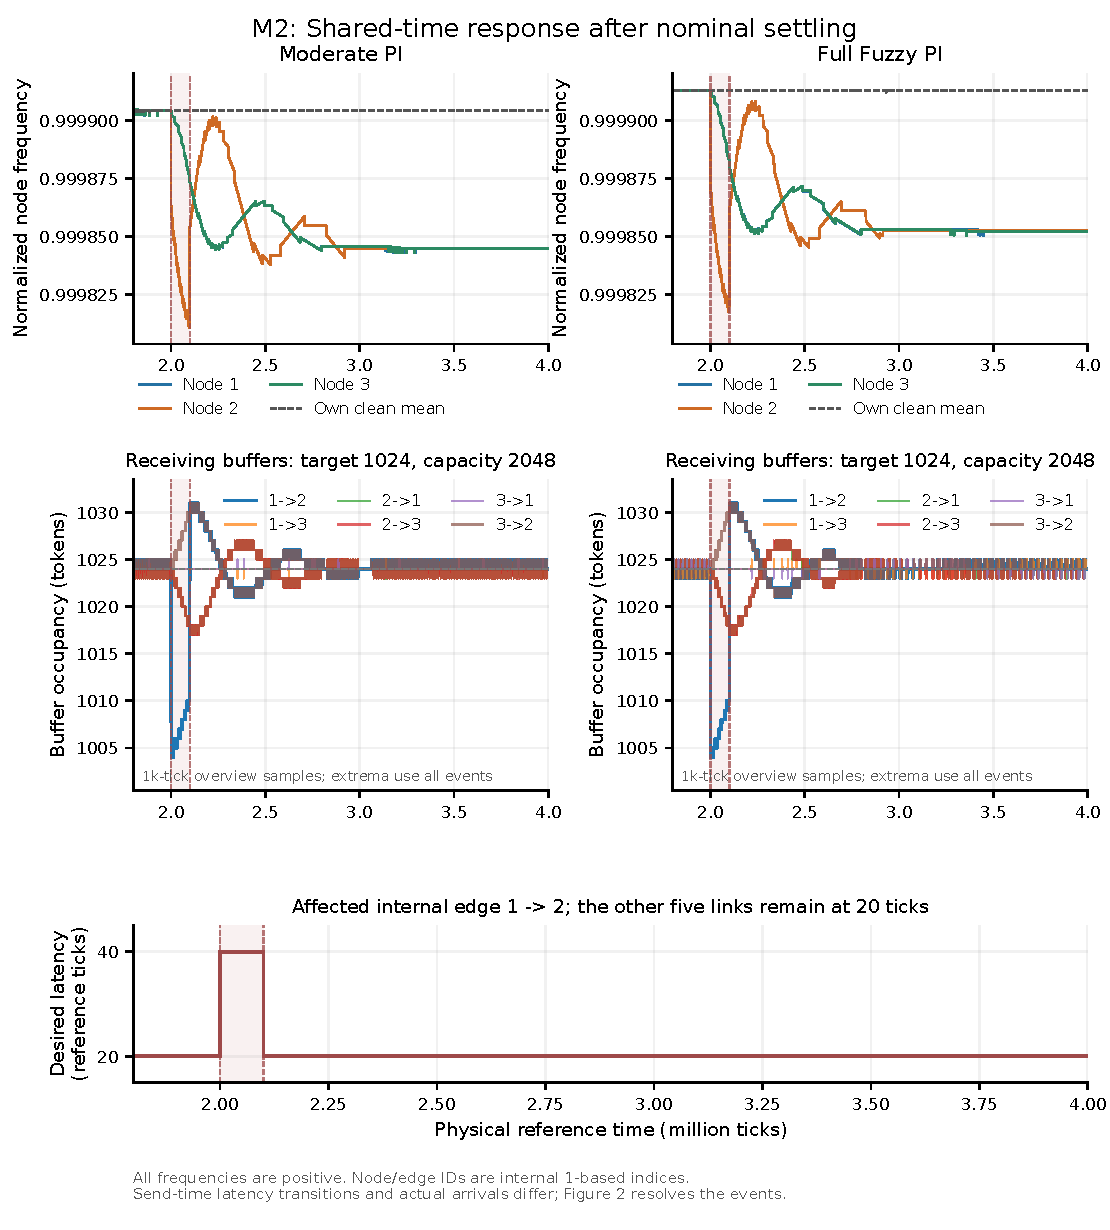
\includegraphics[width=0.97\textwidth]{images/evaluation_20261103/m2_shared_time_response.pdf}
\caption{Aligned post-centering burst experiment. Continuous-phase Callisto
uses the fixed moderate PI coordinates and their full-Fuzzy calibration.
Both controllers have their own clean counterfactual. Desired latency on
one directed channel changes from 20 to 40 during
$[2\times10^6,2.1\times10^6)$. Frequency histories use held corrections;
buffer overview samples are for display, while reported buffer statistics
come from the complete reconstructed event stream.}
\Description{Shared-time overview of node frequencies, six receiving-buffer
occupancies, and the imposed path-latency burst for PI and Fuzzy PI.}
\label{fig:eval_burst_overview}
\end{figure*}

Both controllers remain within capacity with positive frequency and
continuing logical phase progress, without recorded guard or saturation
intervention. Including startup, the full-run maximum deviation is
24 frames for PI and 21 for Fuzzy. This is a favorable Fuzzy endpoint
for that full window, whereas the post-onset peaks are 20 and 21.
Changing the window changes the ranking, so neither figure is used as
a replacement for the other. Capacities are far from exhaustion.

Both first enter the window-qualified component recovery band at
$2.9\times10^6$ and confirm it at $3.2\times10^6$. Thus the experiment
does not show faster Fuzzy settling under this criterion. Strict
own-clean recovery is censored for both. In the memory-diagnostic
tail, the common-frequency changes relative to own clean are
$-59.40198$ ppm for PI and $-60.51069$ ppm for Fuzzy. A stationary
common frequency, frequency agreement between nodes, return to own
clean, and return to frequency one are different properties.

\subsection{Observed nonlinear mechanism and the first buffer peak}
\label{subsec:eval_mechanism}

The M2 rule replay agrees with the full nonlinear implementation.
All sampled Fuzzy input pairs remain in $\Omega_5$, with disturbance-window
maximum $|X|+|Y|=2.001888$. The central identity of
Proposition~\ref{prop:fpi_central} therefore applies to those observed
updates. However, this trajectory does not stay in the smaller
$\Omega_1$ input diamond used by the reference example. This is not
evidence of a sector violation or instability; it is another reason,
besides asynchrony, delay and quantization, that the example's
invariant-region certificate is not a certificate for this actual burst.

The Section~\ref{sec:fpi_controller} decomposition into proportional,
integral-like and accumulated nonlinear-residual terms reproduces the
requested correction with maximum residual approximately
$6.46\times10^{-18}$. In the diagnostic tail, the Fuzzy own-clean
common-frequency shift decomposes into
\begin{equation}
 -60.51069=-57.61859-2.89210\quad\mathrm{ppm},
 \label{eq:eval_memory_accounting}
\end{equation}
where the two terms are the linear integral-like contribution and
nonlinear memory; the proportional contribution is zero. PI's
$-59.40198$ ppm shift is its integral contribution. This is exact
same-trajectory accounting up to numerical arithmetic, not an
independently evolving $F_0$ closed-loop ablation or a unique causal
explanation of the physical common frequency.

Figure~\ref{fig:eval_mechanism} also resolves the first buffer peak.
PI and Fuzzy first attain their disturbance-window maximum target deficits at
ON$+39.105$ and ON$+40.731$ ticks, whereas their first changed commands
relative to own clean occur at ON$+155.216$ and ON$+155.841$.
At the respective first extrema, clean/burst occupancies are
1024/1004 for PI and 1023/1003 for Fuzzy. Both same-time
clean-minus-burst deficits are therefore 20 frames: target deficits of
20 and 21 combine that delivery deficit with clean-state offsets of
zero and one. Consequently the first attainment is not a measurement
of post-burst feedback effectiveness. The minimum is revisited later;
we do not claim that every peak instance precedes feedback.

\begin{figure*}[t]
\centering
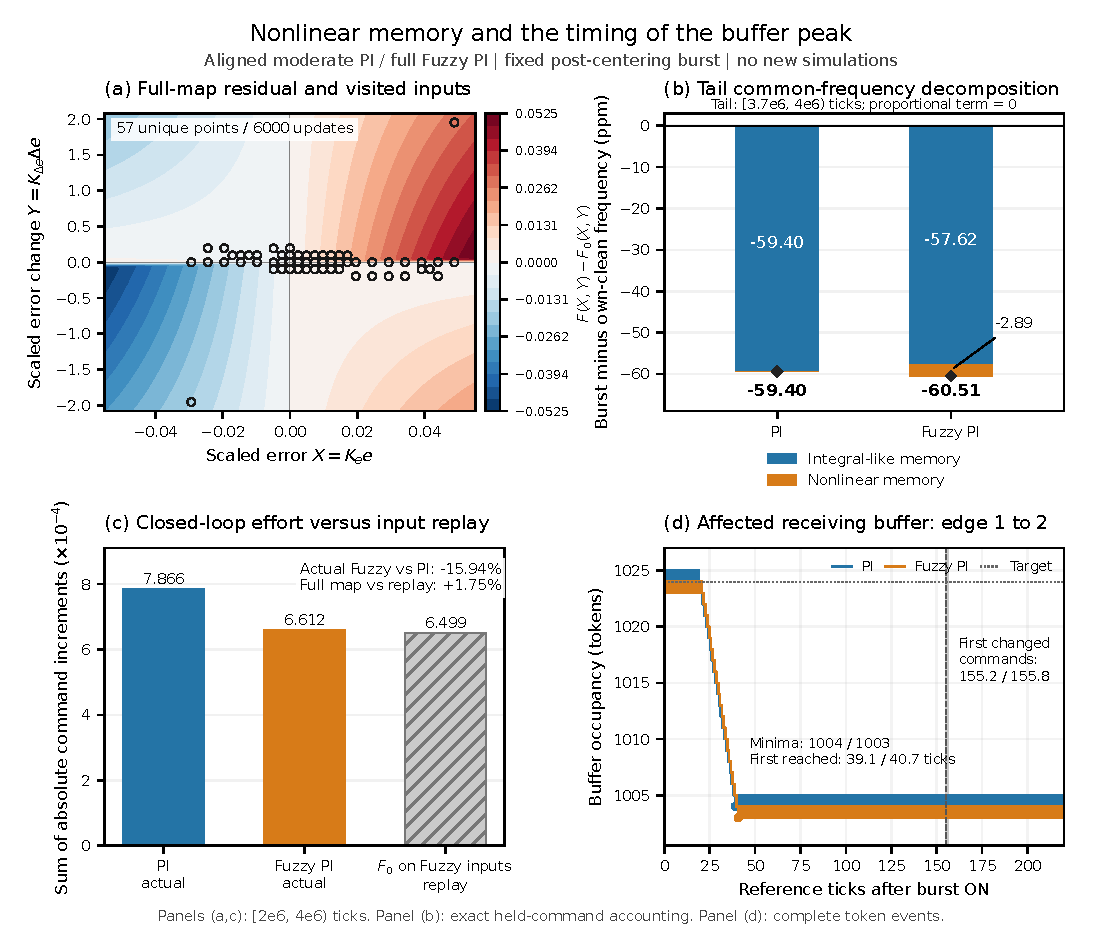
\includegraphics[width=0.97\textwidth]{images/evaluation_20261103/m2_nonlinear_memory.pdf}
\caption{Nonlinear mechanism diagnostics reusing the four M2 runs.
The panels show the exact central residual $F-F_0$, common-frequency
memory accounting, command activity and complete early buffer events.
The hatched $F_0$ activity bar is a replay on Fuzzy's measured inputs,
not a third closed-loop experiment. The residual surface is multiplied
by negative $K_u$ in the controller. The memory panel uses
$[3.7\times10^6,4\times10^6)$; activity uses the main disturbance
window. First peak attainment precedes the first changed command, but
the peak can be revisited after feedback begins.}
\Description{Four panels connecting Fuzzy rule residuals, stored correction
memory, command total variation, and early buffer depletion timing.}
\label{fig:eval_mechanism}
\end{figure*}

\subsection{Independent paired random-latency validation}
\label{subsec:eval_random}

All 180 M3 validation runs are normal-admissible, with zero saved-state
mismatches in complete-event replay. Table~\ref{tab:eval_random}
summarizes the primary endpoint. The ratio estimand is
\begin{equation}
 \widehat r=\frac1{30}\sum_{s=1}^{30}
       \frac{R_{W,s}^{\rm Fuzzy}}{R_{W,s}^{\rm PI}},
 \label{eq:eval_paired_ratio}
\end{equation}
where $s$ indexes independent seeds. It is not the ratio of the two
group means. Pointwise 95\% confidence intervals (CIs) use 20,000
paired-seed percentile-bootstrap resamples with fixed resampling seeds.
Time points, edges and bootstrap draws are not independent experimental
replications. Regimes are analyzed separately; the intervals do not
provide simultaneous multiple-endpoint coverage. There are no excluded
pairs in the reported comparisons.

\begin{table*}[t]
\caption{M3 primary disturbance-window disagreement RMS. Controller entries
are means over 30 seeds in ppm. Ratios are means of paired seed ratios
with pointwise 95\% CIs. A ratio below one favors Fuzzy.}
\label{tab:eval_random}
\centering
\begin{tabular}{@{}lrrrll@{}}\toprule
Profile grid & PI moderate & PI stronger & Fuzzy & Fuzzy/moderate [CI] & Fuzzy/stronger [CI]\\\midrule
$T_c=1000$ & 4.911 & 9.347 & 5.856 & 1.1925 [1.1722,1.2150] & 0.6266 [0.6155,0.6389]\\
$T_c=10000$ & 6.696 & 9.699 & 7.152 & 1.0679 [1.0624,1.0736] & 0.7365 [0.7184,0.7554]\\\bottomrule
\end{tabular}
\end{table*}

\begin{figure*}[t]
\centering
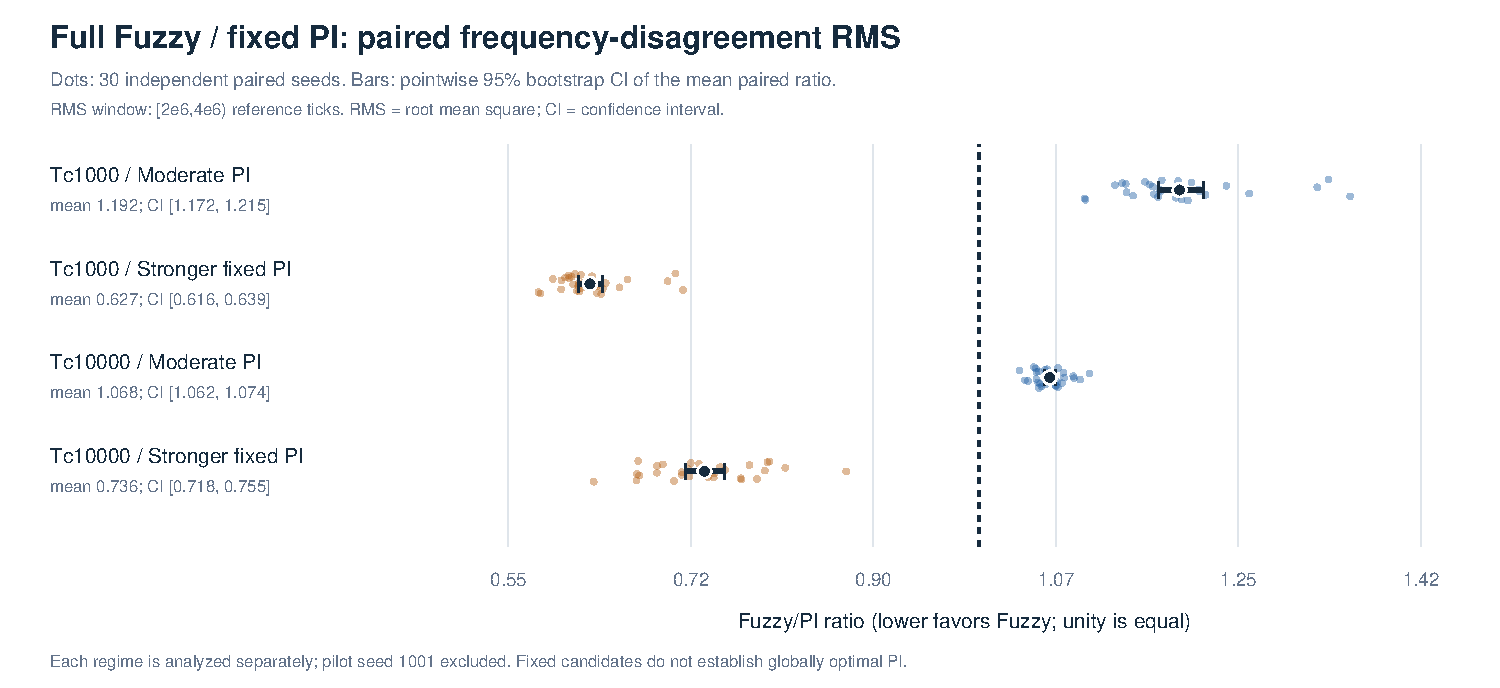
\includegraphics[width=0.97\textwidth]{images/evaluation_20261103/m3_primary_paired_effects.pdf}
\caption{Independent paired random-latency validation: primary disagreement
RMS and paired Fuzzy/PI effects for two physical profile grids. Thirty
seeds per regime are shared across the three fixed controllers. The
moderate comparator is the primary axis-matched PI baseline; stronger
PI is a separate fixed candidate. Ratios and pointwise confidence
intervals follow the paired-seed protocol, rather than resampling
correlated controller updates.}
\Description{Primary random-latency disagreement results and paired effects
against moderate and stronger fixed PI for thirty seeds per regime.}
\label{fig:eval_random_primary}
\end{figure*}

Relative to moderate PI, Fuzzy has higher RMS in all 30 seeds of each
regime: mean paired increases are 19.245\% and 6.791\%. The lower
RMS relative to stronger fixed PI is comparator-specific; moderate PI
already has lower RMS than Fuzzy, so that comparison does not establish
an inherent advantage of fuzzy inference over suitable PI tuning.
The frozen random-latency hypothesis of lower disagreement RMS is
therefore not supported against the primary baseline in these regimes.

Within the disturbance windows, all runs have at most seven frames of
actual target deviation and at least 1017 frames of lower/upper
headroom. These extrema exclude startup. They establish finite-run
admissibility in this interior operating region, not a larger Fuzzy
safe set. The random result also does not extend the M2 TV reduction:
mean paired Fuzzy/moderate TV ratios are 1.03045 and 1.03153.
Figure~\ref{fig:eval_random_secondary} retains buffer, effort and
common-frequency diagnostics. Mean tail common-frequency shifts from
each controller's pre-disturbance level are approximately
$-156.682$ versus $-72.576$ ppm at $T_c=1000$, and $-76.540$
versus $-67.816$ ppm at $T_c=10000$ (Fuzzy versus moderate PI).
These finite-horizon shifts and trends are reported separately from
relative synchronization; no absolute-frequency loop is present.

\begin{figure*}[t]
\centering
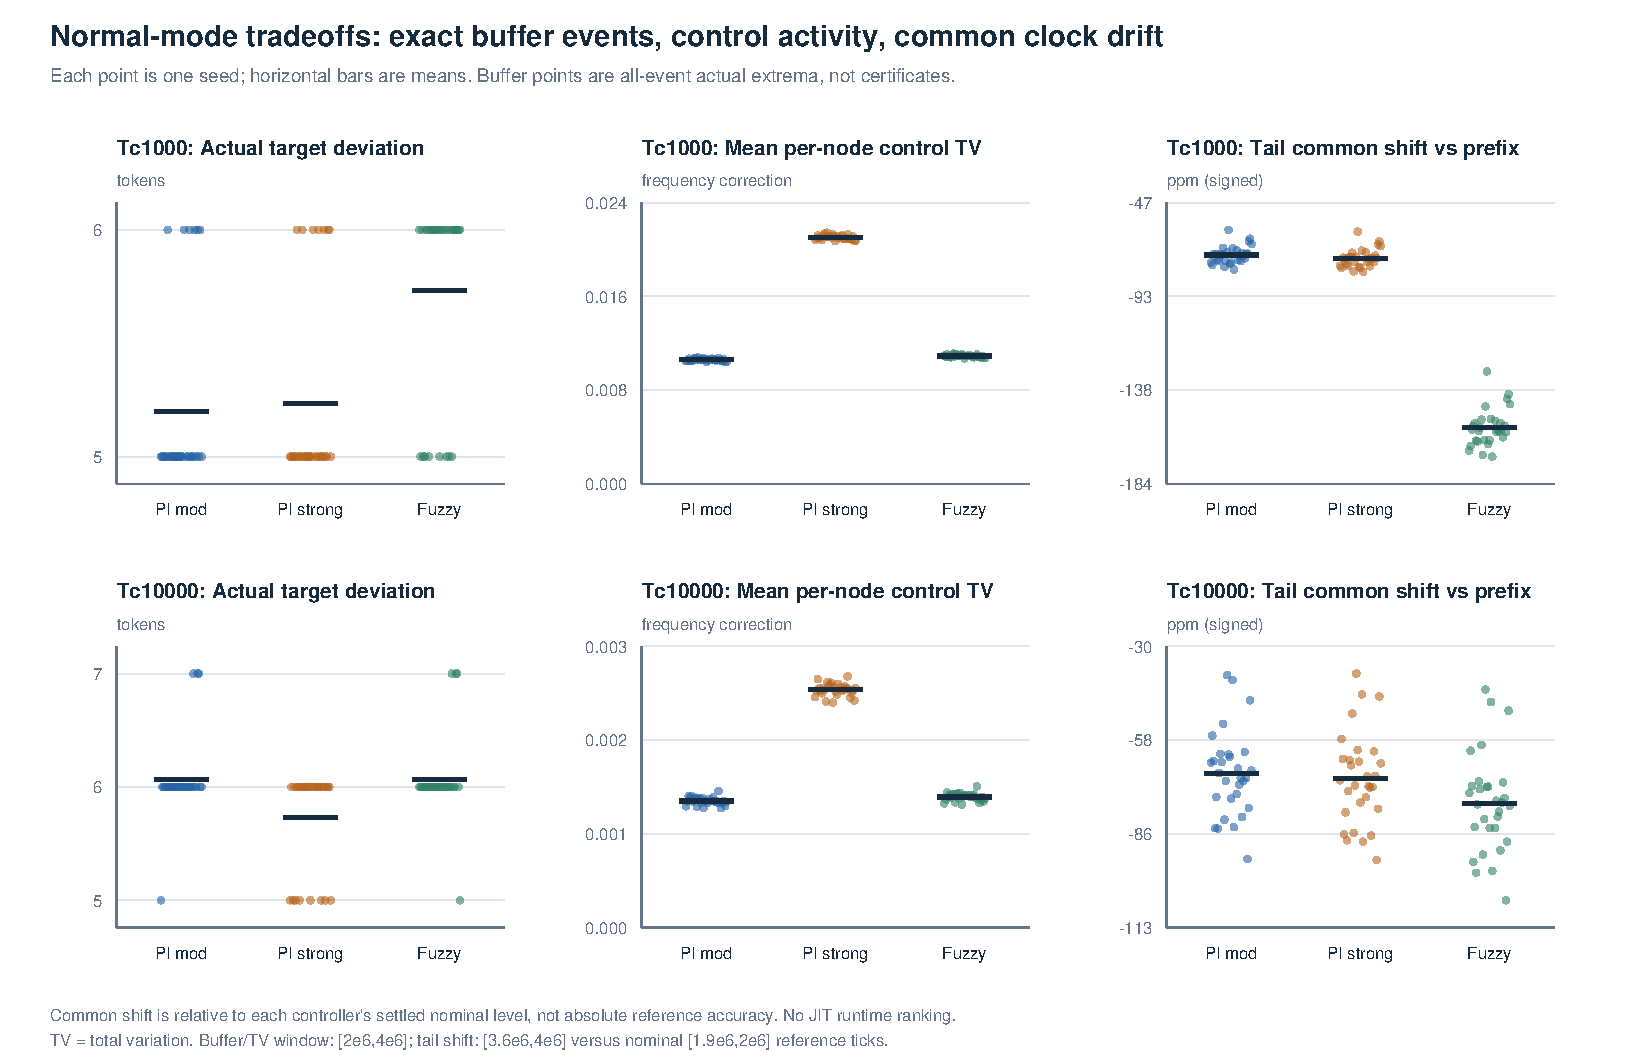
\includegraphics[width=0.97\textwidth]{images/evaluation_20261103/m3_buffer_effort_drift.pdf}
\caption{Secondary M3 diagnostics over the declared windows: complete-event
buffer excursions, command activity and common-frequency shift.
The same 30 paired seeds underlie each regime; additional endpoints
do not create additional independent replications. Buffer extrema
refer to the disturbance window, not the startup trajectory.}
\Description{Buffer, control activity and common-frequency diagnostics
complementing the primary random-latency synchronization metric.}
\label{fig:eval_random_secondary}
\end{figure*}

\subsection{What the completed evaluation establishes}
\label{subsec:eval_support}

The evidence supports the implementation-consistent PI calibration,
the exact nonlinear mechanism on observed M2 inputs, and the
conditional reference-model buffer-headroom theorem. Actual Callisto
demonstrates endpoint-dependent response shaping: a smaller full-run
buffer excursion and lower post-burst IAE/TV at the stated M2 point,
alongside higher post-onset peaks and no faster component recovery.
The independent M3 study limits any general random-jitter advantage
claim for the frozen controller. These outcomes are consistent with
the paper's conditional mechanism-and-tradeoff formulation; they do
not support uniform Fuzzy superiority.

The completed actual campaigns do not test the boundary of the
reference invariant set. Their large buffer reserves cannot substitute
for certified-safe, uncertified-but-observed-safe and failed cases
around a common boundary. Nor do finite observations prove
infinite-horizon safety or the reference theorem's optional
frequency-spread tolerance in asynchronous delayed execution.
Observed phase progress and capacity compliance support normal model
execution; application-payload correctness and a formal refinement
proof of logical synchrony are outside this evaluation.

Finally, these are fixed-controller comparisons, not a completed
equal-budget tuning/held-out-test study. A separate preregistered
tuning campaign has not completed its audit, selection and untouched
tests; its partial results are excluded from the present performance
tables. The evaluation also provides no P/GABA comparison, switched
FFP or observer result, dropout recovery, serialized-link hardware
test, or meaningful controller runtime/energy ranking. Consequently,
practical adoption beyond the reported operating points remains an
empirical question even though the reference-model headroom benefit
is mathematically established.
